\documentclass{article}
\usepackage{graphicx} % Required for inserting images
\usepackage[italian]{babel}
\usepackage[hidelinks]{hyperref}
\usepackage{todonotes}
\usepackage{biblatex}
\usepackage{listings}
\usepackage{parskip}
\usepackage{xurl}


\title{
    Project Management \\
    \textbf{ 
        Planning Approch \\
        for Web Application: \\
        \textit{Google CookBook}
    }
}
\author{
    Marica Pasquali \\ 
    (\href{mailto:marica.pasquali@studio.unibo.it}{marica.pasquali@studio.unibo.it})
}

\begin{document}

\maketitle 
\newpage
\tableofcontents 
\newpage

\section{Scrum}

Scrum è un framework agile per la gestione del ciclo di sviluppo del software, iterativo ed incrementale, concepito 
per gestire progetti e prodotti software o applicazioni di sviluppo.

Scrum prevede la divisione del progetto in blocchi rapidi di lavoro, detti \textit{Sprint}, alla fine di ciascuno 
dei quali viene creato un incremento del software. 

Il vantaggio di questa metodologia è che il Team Scrum rilascia il software in tempo. 
Non serve più aggiornare l'azienda sull'avanzamento del lavoro: basta mostrarglielo! 
I Team Scrum tendono anche a essere più sani degli altri, perché soffrono meno lo stress e registrano 
un tasso di abbandono inferiore grazie alle pratiche Scrum, come la pianificazione degli sprint e le retrospettive 
sprint, che si concentrano sulla preparazione dei colleghi per il successo.


Di seguto è illustrato il processo e i vari componenti della metodologia Scrum.

\begin{figure}[h]
    \centering
    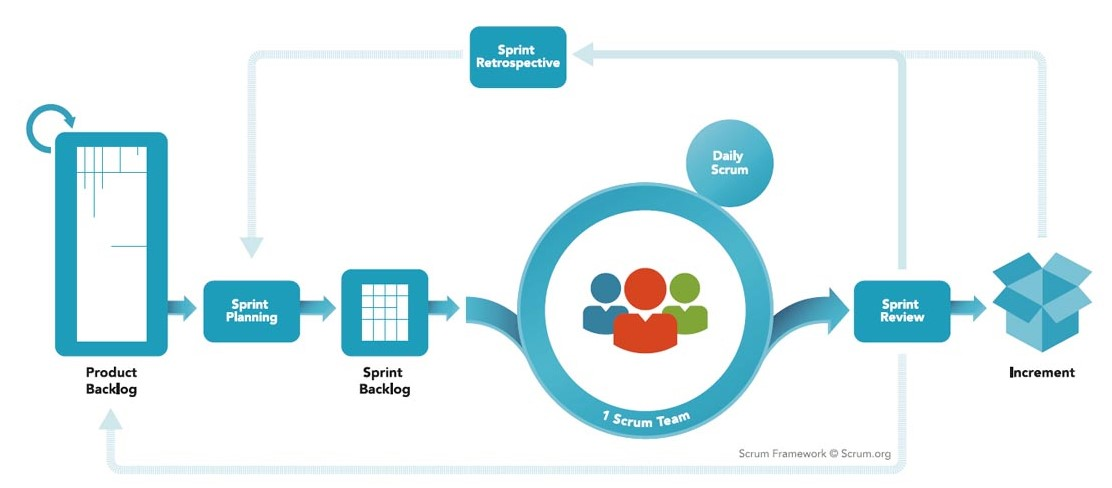
\includegraphics[width=\textwidth]{./imgs/scrum-process.jpg}
\end{figure}


\subsection{Sprint Planning}

Ogni Sprint è preceduto da una riunione di pianificazione, detta \textit{Sprint Planning}, in cui vengono identificati 
gli obiettivi e vengono stimati i tempi.
Durante uno Sprint non è permesso cambiare gli obiettivi, quindi le modifiche sono sospese fino al successivo Sprint Planning, 
e potranno essere prese in considerazione nel successivo Sprint.
Al termine di ogni Sprint il team di sviluppo consegna una versione potenzialmente completa e funzionante del prodotto, 
contenente gli avanzamenti decisi nella riunione di pianificazione dello Sprint.
Nel corso di ogni Sprint, il team crea porzioni complete di un prodotto. 
L'insieme delle funzionalità che vengono inserite in un determinato Sprint provengono dal \textit{Product Backlog}. 
La selezione di quali item del backlog verranno effettivamente inseriti nello Sprint viene effettuata durante lo Sprint Planning meeting. 
Durante questo meeting, il \nameref{product-owner} comunica al team quali item del Product Backlog vorrebbe che fossero completati (quelli con più alta priorità). 
Il team determina quindi quanti di questi pensa di poter completare durante il prossimo Sprint e registra questo dato nello \textit{Sprint Backlog}.
Lo Sprint Backlog è di esclusiva proprietà del team di sviluppo, quindi durante uno Sprint la modifica dello Sprint Backlog non è consentita 
a nessun altro ad eccezione del team di sviluppo. 
Lo sviluppo è di durata fissa, in modo tale che lo Sprint termini alla data prefissata; se i requisiti non sono stati completati 
per una qualsiasi ragione vengono esclusi dalla review e reinseriti nel Product Backlog, a discrezione del Product Owner.

\subsection{Daily Scrum}

Il \textit{Daily Scrum} è un evento della durata massima di 15 minuti che viene effettuato tutti i giorni e 
serve al team di sviluppo per sincronizzare le attività. Questo è fatto controllando il lavoro svolto dopo 
l'ultimo Daily Scrum e prevedendo il lavoro che si svolgerà fino al prossimo incontro.

Il Daily Scrum migliora la comunicazione, elimina altri incontri, identifica e rimuove gli ostacoli allo
sviluppo, evidenzia e promuove il rapido processo decisionale e migliora il livello di conoscenza del
progetto da parte del team di sviluppo. Rappresenta un incontro chiave d'ispezione e adattamento.

\subsection{Sprint Review}
Alla fine dello Sprint si tiene l'incontro di \textit{Sprint Review} per ispezionare l'incremento e adattare, se
necessario, il Product Backlog. Durante la riunione di Sprint Review lo Scrum Team e gli Sponsors
collaborano su ciò che è stato fatto durante lo Sprint. A partire da questo e dai cambiamenti apportati al
Product Backlog durante lo Sprint, i partecipanti collaborano sulle prossime cose che potrebbero essere
fatte per ottimizzare il valore. Si tratta di un incontro informale e la presentazione dell'incremento ha lo
scopo di suscitare commenti e promuovere la collaborazione.

\subsection{Sprint Retrospective}
La \textit{Sprint Retrospective} è un'occasione per lo Scrum Team per ispezionare se stesso e creare un piano di
miglioramento da attuare durante il prossimo Sprint. Lo Scrum Team si riunisce per la Sprint Retrospective dopo 
la Sprint Review e prima del successivo Sprint Planning.

\newpage
\subsection{Artefatti}
Nella metodologia Scrum non c'è la necessità di creare la Work Breakdown Structure (WBS) 
perché può essere sostituita dal \textit{Product Backlog} e dal \textit{Sprint Backlog}.

\subsubsection{Product Backlog}
Il \textit{Product Backlog} è una lista ordinata di tutto ciò che deve essere, o vorresti che venisse, fatto.

Si deve considerarla come una sorta di lista dei desideri in cui sai già da subito che solo una
parte di quello che c'è nel Backlog potrà effettivamente essere fatto.

Si precisa che un task è definito come completato (DONE) quando tutti i test implementati passano 
ed è stata redatta la relativa documentazione.

Il Product Backlog redatto è disponibili nei documenti in allegato.

Tuttavia, essendo un processo iterativo, alcuni aspetti delle attività, dei processi e delle features 
possono cambiare, o addirittura possono emergere delle nuove caratteristiche che non erano state 
pianificate in principio.

\subsubsection{Sprint Backlog}
Lo \textit{Sprint Backlog} è l'insieme degli elementi del Product Backlog selezionati per lo Sprint. 
Lo Sprint Backlog è una previsione fatta dal team di sviluppo in relazione al lavoro necessario 
per rilasciare le funzionalità che saranno presenti nel prossimo incremento, basandosi sulla 
definizione di ``DONE".

Lo Sprint Backlog è un piano con dettagli sufficienti affinché i cambiamenti in atto possano 
essere compresi nel Daily Scrum. Il team di sviluppo modifica lo Sprint Backlog durante
tutto lo Sprint e lo Sprint Backlog emerge durante lo Sprint. 
Quando del nuovo lavoro risulta necessario, il team di sviluppo lo aggiunge allo Sprint Backlog. 
Quando del lavoro viene eseguito o completato, la stima relativa al lavoro rimanente viene aggiornata. 
Se alcuni elementi del piano non sono più ritenuti utili, sono rimossi. 

Solo il team di sviluppo può cambiare il suo Sprint Backlog nel corso di uno Sprint. 
Lo Sprint Backlog è l'immagine prodotta in tempo reale e altamente visibile del lavoro che il team 
di sviluppo prevede di compiere durante lo Sprint; è di esclusiva appartenenza del team di sviluppo.

In qualsiasi momento durante uno Sprint, tutto il lavoro rimanente nello Sprint Backlog può essere
sommato. Il team di sviluppo tiene traccia della quantità di lavoro rimanente quantomeno ad ogni Daily
Scrum. Tenendo traccia del lavoro rimanente attraverso lo Sprint, il team di sviluppo è in grado di
gestire il proprio avanzamento.

\subsubsection{Incremento}
L'\textit{incremento} è la somma di tutti gli elementi del Product Backlog completati durante uno Sprint e
durante tutti gli Sprint precedenti. Alla fine di uno Sprint, il nuovo incremento deve risultare ``DONE", 
il che significa che deve essere utilizzabile e deve incontrare la definizione di ``DONE" data dallo Scrum
Team. Deve essere utilizzabile indipendentemente dal fatto che il Product Owner decida di rilasciarlo
realmente o meno.

\newpage
\subsection{Scrum Team}
Lo Scrum Team è formato da un \textit{Product Owner}, dal \textit{Team di Sviluppo} e da uno \textit{Scrum Master}. 
Gli Scrum Team sono auto-organizzati e cross-funzionali. I Team auto-organizzati scelgono come meglio compiere
il lavoro invece di essere diretti da altri al di fuori del team. I Team cross-funzionali hanno tutte le
competenze necessarie per realizzare il lavoro senza dover dipendere da nessuno al di fuori del team. Il
modello di team in Scrum è progettato per ottimizzare la flessibilità, la creatività e la produttività.
Gli Scrum Team rilasciano i prodotti in modo iterativo e incrementale, massimizzando le opportunità di
feedback. 

\begin{figure}[htbp]
    \centering
    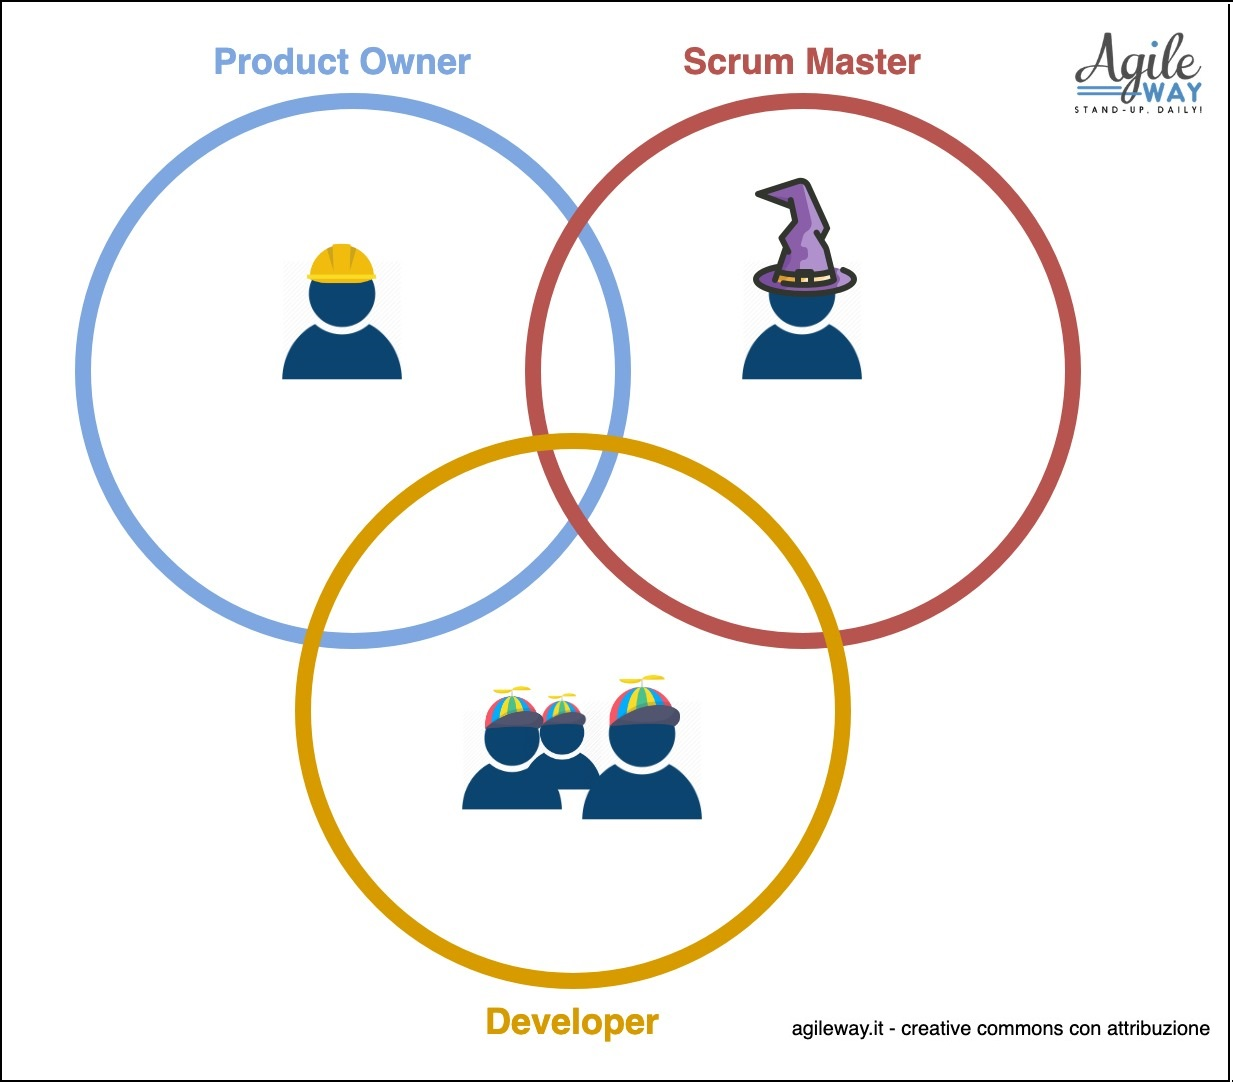
\includegraphics[width=\textwidth]{./imgs/scrum-team.jpg}
    \caption{Scrum Team}
\end{figure}

\newpage
\subsubsection{Product Owner}\label{product-owner}
Il Product Owner è la persona che ha la responsabilità di massimizzare il valore del prodotto e del lavoro svolto dal team di sviluppo 
e la responsabilità esclusiva di gestione del Product Backlog, ossia decide quali attività mettere in cima in base al valore di business, 
ma in pratica il termine ``valore'' può essere talmente soggettivo da essere influenzato dai desideri e le aspettative degli Sponsors, 
da strategie e obiettivi, da rischi, benefici e miglioramenti che si intendono apportare al prodotto.
Il Product Owner è diverso dal tradizionale Product Manager in quanto interagisce attivamente con il team, ne gestisce 
le priorità e ne esamina il lavoro, piuttosto che delegare tutte le decisioni relative allo sviluppo ad un Project Manager. 
Affinché il Product Owner abbia successo, l'intera organizzazione deve rispettare le sue decisioni relative al prodotto. Decisioni che 
sono rese trasparenti e visibili attraverso l'ordinamento del Product Backlog.

\subsubsection{Team di sviluppo}
Il team di sviluppo costruisce il prodotto e le funzionalità indicate dal Product Owner attraverso il Product Backlog. 
Questo team include al suo interno tutto un insieme di skill che sono necessarie allo svolgimento del progetto, senza dover dipendere da team esterni. 
Come già detto in precedenza il team è anche autogestito e gode di un alto livello di autonomia e di responsabilità.
All'inizio di ciascuno Sprint il Product Owner espone le priorità e il team decide autonomamente su quali attività impegnarsi, facendo il possibile 
per raggiungere il risultato con le modalità di lavoro che ritiene adeguate.
Il Team non solo sviluppa quanto richiesto, ma dà anche indicazioni e suggerimenti al Product Owner al fine di migliorare il prodotto e renderlo ottimale.
In Scrum si ottengono i risultati migliori quando il team è dedicato al 100\% sul progetto. 


\subsubsection{Scrum Master}
Lo Scrum Master ha il compito di aiutare il team ad essere efficace e a raggiungere gli obiettivi attraverso la pratica di Scrum. 
E' una figura chiave nel facilitare il gruppo a risolvere gli impedimenti e nel proteggerlo da ogni rumore esterno durante lo Sprint.
Lo Scrum Master è un vero leader a servizio non solo del team ma anche dell'organizzazione.
Un buon Scrum Master educa e guida l'intero gruppo di lavoro all'uso di Scrum e fa in modo che chiunque, inclusi il Product Owner e il management 
dell'azienda, ne comprendano e ne seguano i principi e le pratiche. È importante che lo Scrum Master sia appassionato e che lavori energicamente 
alla risoluzione degli impedimenti che possono compromettere la riuscita di uno Sprint o di un intero progetto.
Il ruolo di Scrum Master (non sempre) è assunto da uno dei membri del gruppo.
A differenza di un Project Manager, lo Scrum Master non assegna task ai membri del team e non dice loro che cosa devono fare, ma facilita il processo 
aiutando il team ad auto gestirsi e organizzarsi.

\newpage
\subsection{Strumenti}

\subsubsection{Scrum Board}
La Scrum Board è una rappresentazione visiva del lavoro che un team Scrum deve svolgere. 
È altrimenti definibile, anche, come un display visivo che traccia i progressi di un progetto su formato fisico o virtuale.
La Scrum Board consiste effettivamente in una lavagna in cui vengono segnati i progressi dello Sprint, dal principio, 
fino al completamento.
Il suo scopo è quello di semplificare l'organizzazione dei progetti e la loro gestione. 
Infatti, tramite la Scrum Board è possibile isolare e organizzare i diversi compiti del gruppo di lavoro, così come monitorare 
ogni singolo task tramite il suo ciclo vita. 

La Scrum Board del seguente progetto è stata suddivisa come segue:
\begin{itemize}
    \item \textbf{Product Backlog}
    \item \textbf{Sprint Backlog}
    \item \textbf{In Progress}
    \item \textbf{In Review}
    \item \textbf{Done}
\end{itemize}

La Scrum Board (in Trello) è disponibile al seguente indirizzo: 

\url{https://trello.com/invite/b/FqVavaID/ATTI3494f46414e79dfea191a74b3917c5dbB108DE50/scrumboard-pm}

oppure utilizzando il QR Code seguente:

\begin{figure}[h]
    \centering
    
\includegraphics[scale=1]{./imgs/trello-board-qr-code.png}
    \caption{QR Code per accedere alla Scrum Board di \textit{Google CookBook} in Trello}
\end{figure}

\newpage
Di seguito viene illustrata una preview della Scrum Board.

\begin{figure}[h]
    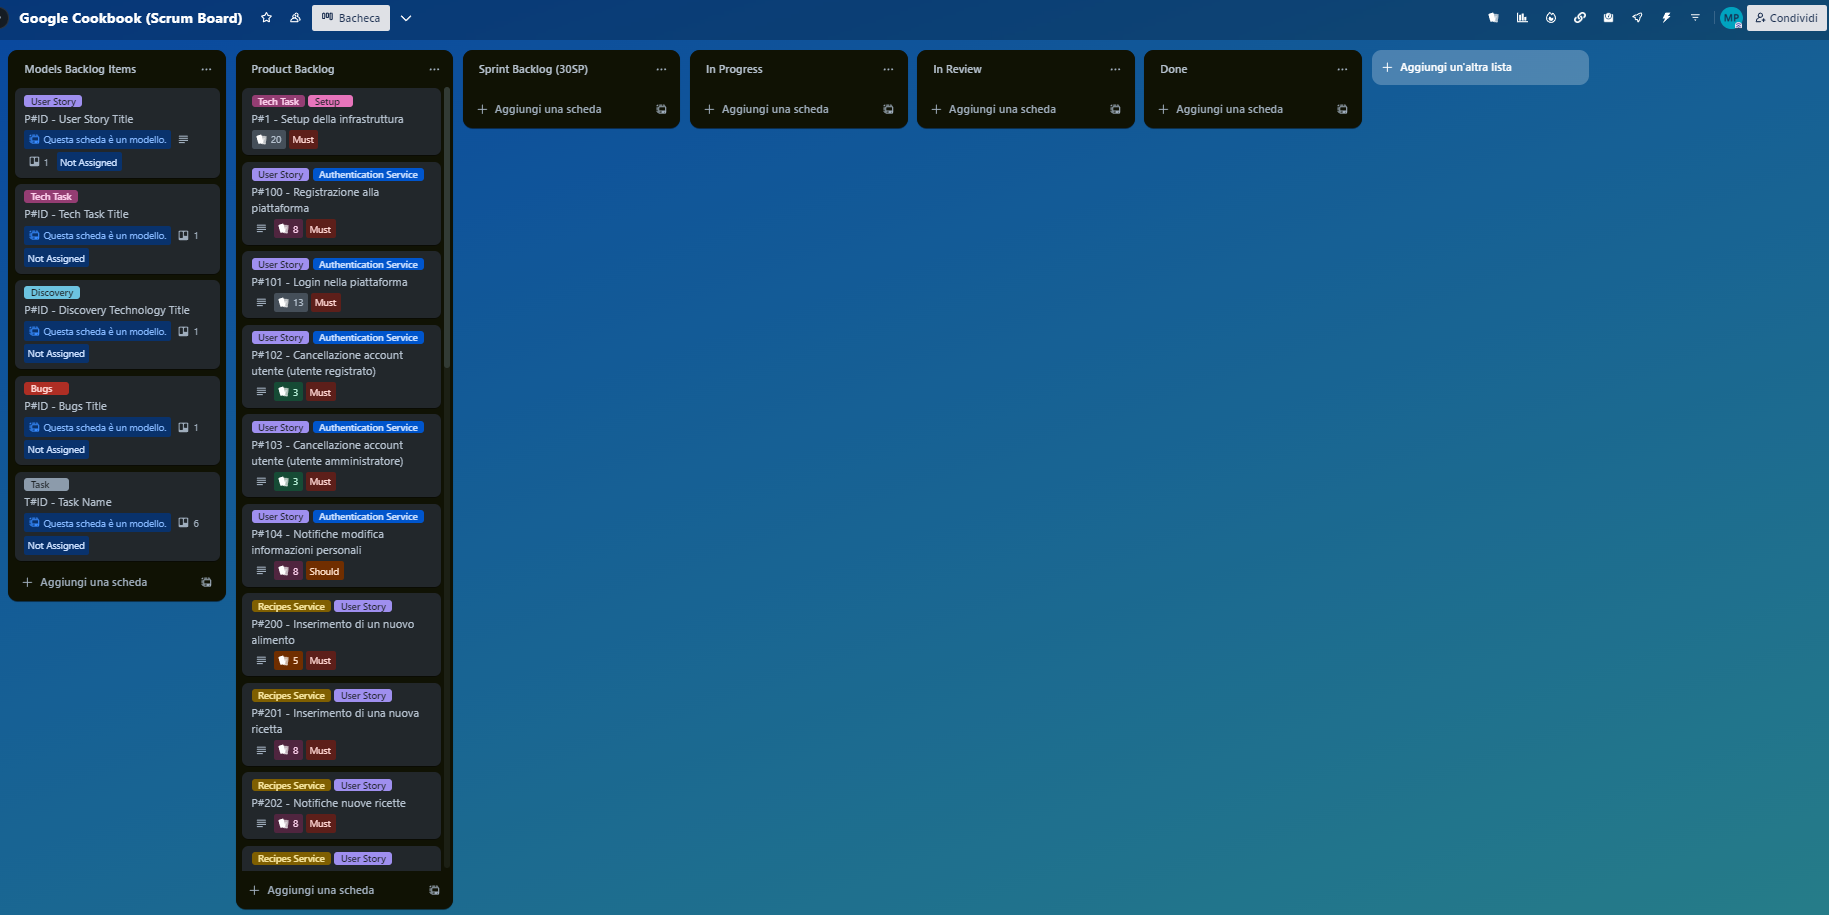
\includegraphics[width=\textwidth]{./imgs/scrum-board.png}
    \caption{Scrum Board di \textit{Google CookBook}}
\end{figure}

\newpage
\section{Stime dei tempi}

La stima dei tempi degli item del Product Backlog è effettuata sulla ``complessità di sviluppo" delle diverse user story, 
che è misurata in story point (SP), misura relativa della dimensione e complessità di una user story.
L'assegnazione degli story point è affettuato tramite la tecnica del 
\href{https://en.wikipedia.org/wiki/Planning_poker}{\textit{Planning Poker (o Scrum Poker)}}, 
in cui i membri del team assegnano gli story point basandosi sull'esperienza e la conoscenza del 
dominio del progetto.
L'uso degli story point è favorito dalla necessità di pianificare ciascuno sprint, selezionando 
il sottoinsieme di user story da mettere in produzione utilizzando gli story point disponibili 
nello sprint.

Al contrario la stima dei tempi dei task ricavati dalle user story è effettuata in termini di sessioni utilizzando 
la \textit{Pomodoro Technique}.


Nel seguente progetto si è deciso che uno Sprint abbia le seguenti caratteristiche:
\begin{itemize}
    \item durata di 2 settimane (ossia 10 giorni lavorativi)
    \item presa in carico di 30 story point. Questa stima può essere abbassata o aumentata dopo 
    ogni sprint nel caso ci sia stato un sovraccarico o sottocarico di lavoro durante lo sprint 
    appena finito
    \item ogni sviluppatore lavora utilizzando la \textit{Pomodoro Technique} ossia 25 minuti in cui 
    lavora senza interruzzioni e distrazioni, intervallati da delle pause di 5 minuti (o anche più lunghe
    dopo un certo numero di blocchi)
\end{itemize}

Una prima stima, indicativa, prevede 8 sprint per una durata complessiva di 16 settimane, tuttavia 
questa stima potrebbe cambiare durante lo svolgimento del progetto.

\end{document}

